\documentclass[11pt]{article}
\usepackage[top=1cm, bottom=2cm, left=1cm, right=1cm]{geometry}
\usepackage{ctex}
\usepackage[linesnumbered,ruled]{algorithm2e}
\usepackage{amsthm,amsmath,amssymb}
\usepackage[colorlinks=true,linkcolor=blue]{hyperref}
\usepackage{listings}
\usepackage{xcolor,xparse}
\usepackage{realboxes}
\usepackage{mathrsfs}
\usepackage{wrapfig}
\usepackage{subfigure}
\usepackage{forest}
\usepackage{pifont}
\usepackage{ulem}
\usepackage{bm}

\SetKw{Print}{print}
\SetKw{Read}{read}
\SetKw{Allocate}{allocate}
\SetKw{Deallocate}{deallocate}
\SetKw{Call}{call}
\SetKw{True}{true}
\SetKw{False}{false}
\SetKw{Continue}{continue}
\SetKw{Break}{break}
\SetKw{Write}{write}

\definecolor{cmdbg}{rgb}{0.9,0.9,0.9}
\lstset{%
	basicstyle=\ttfamily,
	breaklines = true,
	backgroundcolor=\color{cmdbg},
}
\DeclareDocumentCommand{\ccmd}{v}{% 参数 v 表示工作方法类似于 \verb
    \Colorbox{cmdbg}{\csname lstinline\endcsname!#1!}%
}


\author{杨远青 22300190015}
\title{计算物理作业3}

\begin{document}
\maketitle
\textit{远方来朋,喜;假期俱至,悦。}

\section{\texorpdfstring{\sout{题目 1:高斯消元法的时间复杂度分析}}{题目 1:高斯消元法的时间复杂度分析}}
\subsection{题目描述}
Prove that the time complexity of Gaussian elimination algorithm is $\mathcal{O}(n^3)$.
\subsection{证明}
Gaussian消元法,此处特指\textit{Forward Elimination} \& \textit{Backward Substitution}法,而不是最古老的Gaussian-Jordan消元法(用于求逆的某浪漫主义教学算法),在大多数情况下的表现,并不如兼具精确度与效率的$\bm{LU}$分解法,但一些思想被嵌入后者与适用于更大规模矩阵求解的各类迭代算法中,因此仍有必要对其进行分析。

先考虑\textit{Forward Elimination}的时间复杂度,即通过初等行变换将原本的增广矩阵
$\bm{(A \, | \, b)}$
\[
	\left[\begin{array}{cccc|c}a_{11}&a_{12}&\cdots&a_{1n}&b_{1}\\a_{21}&a_{22}&\cdots&a_{2n}&b_{2}\\\vdots&\vdots&\ddots&\vdots&\vdots\\a_{n 1}&a_{n 2}&\cdots&a_{n n}&b_{n}\end{array}\right]
\]
上三角化为$\bm{U}$。暂不考虑\textit{Pivot}步骤可能带来的交换操作,尽管这对于提升数值稳定性非常重要。考虑第$1$列的第$2$至$n$行,每一行需要先计算系数$a_{i1}/a_{11}$,再进行$n$次乘法与$n$次减法(各行首元素直接设为$0$,不计入乘减法操作,但要考虑最右侧$b$的元素),故第$1$列的消元操作数为$(n-1)(2n+1)$,递推可知,第$i$步便是对$(n-i+1)\times(n-i+1)$子矩阵的消元,迭代操作数为$(n-i)(2n-2i+3)$,总操作数为
\[
	T_F(n) =
	\sum_{i=1}^{n-1} (2n-2i+3)(n-i) = 2\sum_{i=1}^{n-1} (n-i)(n-i)+3\sum_{i=1}^{n-1} (n-i) = \frac{4n^3+3n^2-7n}{6}.
\]
再考虑\textit{Backward Substitution}的时间复杂度,当我们消元得到一个$n \times n$的上三角矩阵$\bm{U}$
\[
	\left[\begin{array}{cccc|c}a_{11}'&a_{12}'&\cdots&a_{1 n}'&b_{1}'\\0&a_{22}'&\cdots&a_{2 n}'&b_{2}'\\\vdots&\vdots&\ddots&\vdots&\vdots\\0&0&\cdots&a_{n n}'&b_{n}'\end{array}\right]
\]
之后,需要从最后一行开始,逐行求解
\[
	x_i=\frac{1}{a_{i i}'}\left(b_i'-\sum_{j=i+1}^ka_{i j}' x_j\right).
\]
每一行涉及的四则运算(我们非常流氓地忽视除法的独特地位,理论上这需要基于牛顿迭代的现代方法进行特殊处理)为$(n-i)$次乘法与$(n-i)$次减法,再进行$1$次除法,故每行的操作数为$[2(n-i)+1]$,总操作数为
\[
	T_B(n)=\sum_{i=1}^n \ [2(n-i)+1]=2\sum_{i=1}^n (n-i)+n=n^2.
\]
故Gaussian消元法的总操作数为
\[
	T(n)=T_F(n)+T_B(n)=\frac{4n^3+3n^2-7n}{6}+n^2=\frac{4n^3+9n^2-7n}{6}.
\]
其中有除法$n(n+1)/2$次,乘法与减法各$n(n-1)(2n+5)/6$次,故
\[
	\boxed{T(n) = \mathcal{O}(n^3)}
\]

伙计,这听起来一点也不酷,怎么到头来还是和求逆矩阵一样是$\mathcal{O}(n^3)$?但如果我们将\textit{Substitution}的思想嵌入到$\bm{LU}$分解法\footnote{详见\textit{Numerical Recipes $\S 2.4$}},对一些特定情形,譬如三对角矩阵的回代操作可以从$\mathcal{O}(n^2)$优化到$\mathcal{O}(n)$,且对于不同的待解向量$\bm{b}$,我们的圣遗物$\bm{L}$和$\bm{U}$可以被重复利用,这听上去还是不错的!

如果想和理论计算机科学家一样,执着于对$\mathcal{O}(n^3)$的优化:Strassen的构造可以帮你将指数因子优化到$\mathcal{O}(n^{\log_2 7})$,即$\omega  = \log_2 7 \approx 2.8074$\footnote{有个直观而有趣的讨论,详见\textit{Numerical Recipes $\S 2.11$}},采用Coppersmith–Winograd矩阵乘法可以优化到$\omega \le 2.3755$\footnote{$\omega < 2.404$的一种证明,参见\ \href{https://people.csail.mit.edu/virgi/6.890/lecture23.pdf}{\textit{MIT6.890 $\S 23$}}}.但这类小数点后的“用力过度”不是我们的菜,有时候反倒是滥用主定理,即它们所需的天文数字规模$N\times N$的矩阵来临时,我们早该另觅出路,比如考虑使用Jacobi等迭代法。

\setcounter{section}{0}
\vspace{1em}
\textit{公元二〇二四年九月二十四日,午时三刻,于HGX106室,惊闻徐夫子欲改弦更张,悲哉!}
\vspace{-1em}
\section{\texorpdfstring{题目 1:$\bm{LU}$分解法的时间复杂度分析}{题目 1:LU分解法的时间复杂度分析}}
\subsection{题目描述}
Prove that the time complexity of $\bm{LU}$ decomposition algorithm is $\mathcal{O}(n^3)$.
\subsection{证明}
$\bm{LU}$分解法的第一步是将系数矩阵$\bm{A}$分解为一个下三角矩阵$\bm{L}$和一个上三角矩阵$\bm{U}$:
\[
    \begin{bmatrix}
        a_{11} & a_{12} & \cdots & a_{1n} \\
        a_{21} & a_{22} & \cdots & a_{2n} \\
        \vdots & \vdots & \ddots & \vdots \\
        a_{n1} & a_{n2} & \cdots & a_{nn}
    \end{bmatrix}
    =
    \begin{bmatrix}
        l_{11} & 0      & \cdots & 0      \\
        l_{21} & l_{22} & \cdots & 0      \\
        \vdots & \vdots & \ddots & \vdots \\
        l_{n1} & l_{n2} & \cdots & l_{nn}
    \end{bmatrix}
    \begin{bmatrix}
        1      & u_{12} & \cdots & u_{1n} \\
        0      & 1      & \cdots & u_{2n} \\
        \vdots & \vdots & \ddots & \vdots \\
        0      & 0      & \cdots & 1
    \end{bmatrix}.
\]
这一步常采用Crout方法实现,即在每一轮中,我们先计算$\bm{L}$的第$k$列元素$l_{ik}$,
\[
    l_{ik} = a_{ik} - \sum_{s=1}^{k-1} l_{is} u_{sk}, \quad \ i = k, k+1, \dots, n.
\]
每一个$l_{ik}$的计算涉及$k-1$次乘法和$k-1$次减法,共有$(n-k+1)$个$l_{ik}$需要计算;再计算$\bm{U}$的第$k$行元素$u_{kj}$,
\[
    u_{kj} = \frac{1}{l_{kk}} \left( a_{kj} - \sum_{s=1}^{k-1} l_{ks} u_{sj} \right), \quad \ j = k+1, k+2, \dots, n.
\]
相比$l_{ik}$的计算多了一次除法,共有$(n-k)$个$u_{kj}$需要计算,故第$k$轮的操作数为
\[
    (n-k+1)\cdot(2k-2)+(n-k)\cdot(2k-1) = -4k^2 + (4n+5)k -3n -2.
\]
因此,分解步骤的总操作数为
\[
    T_c(n) =\sum_{k=1}^{n} \ [-4k^2 + (4n+5)k -3n -2]                                                 \\
    = -4 \cdot \frac{n(n+1)(2n+1)}{6} + (4n+5) \cdot \frac{n(n+1)}{2} - (3n+2) \cdot n\\
    = \frac{4n^3 - 3n^2 - n}{6}.
\]

再考虑回代步骤的操作数,即用分解得到的$\bm{L}$和$\bm{U}$求解方程组$\bm{Ax} = \bm{b}$。首先求解$\bm{Ly} = \bm{b}$,即
\[
    \begin{bmatrix}
        l_{11} & 0      & \cdots & 0      \\
        l_{21} & l_{22} & \cdots & 0      \\
        \vdots & \vdots & \ddots & \vdots \\
        l_{n1} & l_{n2} & \cdots & l_{nn}
    \end{bmatrix}
    \cdot
    \begin{bmatrix}
        y_1 \\ y_2 \\ \vdots \\ y_n
    \end{bmatrix}
    =
    \begin{bmatrix}
        b_1 \\ b_2 \\ \vdots \\ b_n
    \end{bmatrix}.
\]
这实质上是从第一行开始的\textit{Forward Substitution},即
\[
    y_i=\frac{1}{l_{i i}}\left(b_i-\sum_{j=1}^{i-1} l_{i j} y_j\right).
\]
每一步有$1$次除法,$(i-1)$次乘法与$(i-1)$次减法;再求解$\bm{Ux} = \bm{y}$,即
\[
    \begin{bmatrix}
        1      & u_{12} & \cdots & u_{1n} \\
        0      & 1      & \cdots & u_{2n} \\
        \vdots & \vdots & \ddots & \vdots \\
        0      & 0      & \cdots & 1
    \end{bmatrix}
    \cdot
    \begin{bmatrix}
        x_1 \\ x_2 \\ \vdots \\ x_n
    \end{bmatrix}
    =
    \begin{bmatrix}
        y_1 \\ y_2 \\ \vdots \\ y_n
    \end{bmatrix},
\]
这实质上是从最后一行开始的\textit{Backward Substitution},即
\[
    x_i=\left(y_i-\sum_{j=i+1}^{n} u_{i j} x_j\right).
\]
每一步有$(n-i)$次乘法与$(n-i)$次减法,故回代步骤操作数为
\[
    T_s(n)=\sum_{i=1}^{n} \ [(2i-1)+(2n-2i)] = \sum_{i=1}^{n} (2n-1) = n(2n-1) = 2n^2 -n.
\]
因此,$\bm{LU}$分解法的总操作数为
\[
    T(n)=T_c(n)+T_s(n)=\frac{4n^3 -3n^2 -n}{6} + 2n^2 -n = \frac{4n^3 +9n^2 -7n}{6}.
\]
其中有除法$n(n+1)/2$次,乘法与减法各$n(n-1)(2n+5)/6$次,故
\[
    \boxed{T(n) = \mathcal{O}(n^3)}
\]
\textit{Amazing,居然与Gaussian消元法的各种操作数都相同!}

\section{题目 2:结合部分主元应用高斯消元法}
\subsection{题目描述}
\noindent Write a code to numerically solve the radial Schrödinger equation for
\[
\left[-\frac{1}{2}\nabla^2+V(\mathbf{r})\right]\psi(\mathbf{r})=E\psi(\mathbf{r}), \quad V(\mathbf{r})=V(r)
\]
\begin{enumerate}
    \item \( V(r) = \frac{1}{r} \) (hydrogen atom)
    \item Considering the following potential:
    \[
    V(r) = -\frac{Z_{\text{ion}}}{r}\text{erf}\left(\frac{r}{\sqrt{2} r_{\text{loc}}}\right) 
    + \exp \left[ -\frac{1}{2} \left(\frac{r}{r_{\text{loc}}}\right)^{\frac{1}{2}}\right]
    \times \left[C_1 + C_2\left(\frac{r}{r_{\text{loc}}}\right)^2+C_3\left(\frac{r}{r_{\text{loc}}}\right)^4+C_4\left(\frac{r}{r_{\text{loc}}}\right)^6\right]
    \]
\end{enumerate}
where \(\text{erf}\) is the error function. And for Li, you could set:
\begin{itemize}
    \item \( Z_{\text{ion}}=3 \)
    \item \( r_{\text{loc}}=0.4 \)
    \item \( C_1=-14.0093922 \)
    \item \( C_2=9.5099073 \)
    \item \( C_3=-1.7532723 \)
    \item \( C_4=0.0834586 \)
\end{itemize}
\noindent Compute and plot the first three eigenstates. You could find more information about 'how to solve radial Schrödinger equation' and 'use of non-uniform grid (optional)' in the PPT.

\textbf{Special Note:} You may call any library functions for diagonalization.


\subsection{程序描述}

\subsection{伪代码}
Powered by \href{https://chatgpt.com/g/g-xJJAA2awf-latex-pseudocode-generator}{\LaTeX \ pseudocode generator}

\subsection{结果示例}



\section{题目 3:变分法求解一维薛定谔方程}
\subsection{题目描述}
\noindent Given \( n+1 \) points \((x_0, y_0), (x_1, y_1), \dots, (x_n, y_n)\), the \( n \)-th order interpolation polynomial using Newton's method is:
\[
P_n(x) = f[x_0] + f[x_1, x_0](x - x_0) + f[x_2, x_1, x_0](x - x_0)(x - x_1) + \cdots + f[x_n, x_{n-1}, \dots, x_0](x - x_0)(x - x_1) \dots (x - x_{n-1})
\]
where \( f[x_i, x_{i-1}, \dots, x_0] \) represents the divided differences. Taking the coefficients from the lower edge of the difference table (i.e., \( f[x_n], f[x_n, x_{n-1}], \dots, f[x_n, \dots, x_0] \)), will this provide higher accuracy for values of \( x \) near \( x_n \)?

\begin{center}
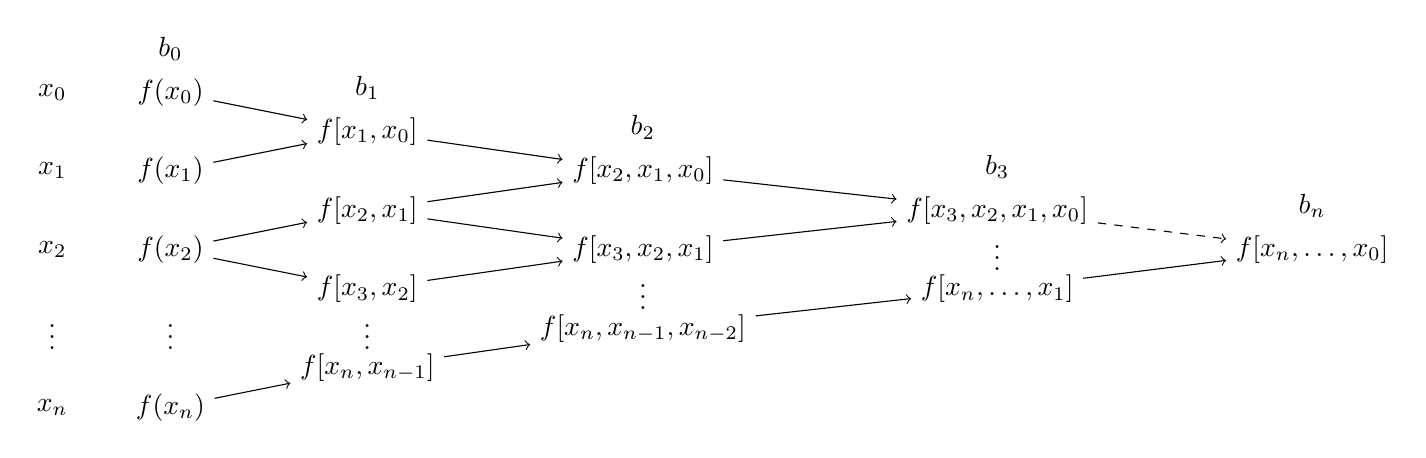
\begin{tikzpicture}
    % Column 1 (x values)
    \node (x0) at (-4, 0) {$x_0$};
    \node (x1) at (-4, -1) {$x_1$};
    \node (x2) at (-4, -2) {$x_2$};
    \node (dots) at (-4, -3) {$\vdots$};
    \node (xn) at (-4, -4) {$x_n$};

    % Column 2 (f(x) values)
    \node (f0) at (-2.5, 0) {$f(x_0)$};
    \node (f1) at (-2.5, -1) {$f(x_1)$};
    \node (f2) at (-2.5, -2) {$f(x_2)$};
    \node (fdots) at (-2.5, -3) {$\vdots$};
    \node (fn) at (-2.5, -4) {$f(x_n)$};

    % Column 3 (f[x1, x0], etc.)
    \node (f10) at (0, -0.5) {$f[x_1, x_0]$};
    \node (f21) at (0, -1.5) {$f[x_2, x_1]$};
    \node (f32) at (0, -2.5) {$f[x_3, x_2]$};
    \node (fdots2) at (0, -3) {$\vdots$};
    \node (fnn1) at (0, -3.5) {$f[x_n, x_{n-1}]$};

    % Column 4 (f[x2, x1, x0], etc.)
    \node (f210) at (3.5, -1) {$f[x_2, x_1, x_0]$};
    \node (f321) at (3.5, -2) {$f[x_3, x_2, x_1]$};
    \node (fdots3) at (3.5, -2.5) {$\vdots$};
    \node (fnnn2) at (3.5, -3) {$f[x_n, x_{n-1}, x_{n-2}]$};

    % Column 5 (f[x3, x2, x1, x0], etc.)
    \node (f3210) at (8, -1.5) {$f[x_3, x_2, x_1, x_0]$};
    \node (fdots4) at (8, -2) {$\vdots$};
    \node (fnnnn3) at (8, -2.5) {$f[x_n, \dots, x_1]$};

    % Column 6 (final term)
    \node (final) at (12, -2) {$f[x_n, \dots, x_0]$};

    % Labels for coefficients
    \node[above=8pt] at (f0) {$b_0$}; % 向上偏移8pt
    \node[above=8pt] at (f10) {$b_1$};
    \node[above=8pt] at (f210) {$b_2$};
    \node[above=8pt] at (f3210) {$b_3$};
    \node[above=8pt] at (final) {$b_n$};

    % Drawing connections with (dashed) lines
    \draw[->] (f0) -- (f10);
    \draw[->] (f10) -- (f210);
    \draw[->] (f210) -- (f3210);
    \draw[dashed, ->] (f3210) -- (final);

    % Drawing vertical solid lines within each column
    \draw[->] (f1) -- (f10);
    \draw[->] (f2) -- (f21);
    \draw[->] (f2) -- (f32);
    \draw[->] (f21) -- (f210);
    \draw[->] (f21) -- (f321);
    \draw[->] (f32) -- (f321);
    \draw[->] (f321) -- (f3210);
    \draw[->] (fn) -- (fnn1);
    \draw[->] (fnn1) -- (fnnn2);
    \draw[->] (fnnn2) -- (fnnnn3);
    \draw[->] (fnnnn3) -- (final);

\end{tikzpicture}
\end{center}

\subsection{程序描述}
原本对于不考虑舍入误差的理想形式,Newton插值与Lagrange插值的结果必定是唯一且等价的,也即通过给定$(n+1)$个节点的$n$阶多项式唯一,这一点可以从Vandermonde行列式
\[
\det \begin{pmatrix}
1 & x_0 & x_0^2 & \cdots & x_0^n \\
1 & x_1 & x_1^2 & \cdots & x_1^n \\
\vdots & \vdots & \vdots & & \vdots \\
1 & x_n & x_n^2 & \cdots & x_n^n
\end{pmatrix} = \prod_{0 \leq i < j \leq n} (x_j - x_i)
\]
非奇异中看出。但实际结果中,我们必须考虑舍入误差,这使得Newton插值的结果可能会依赖于节点的顺序。尤其是在我们使用Horner's Rule(\ref{eq:horner})的时候,显然在节点附近的插值数值稳定性依赖于节点的顺序。本程序使用\ref{sec:problem_1}节中的牛顿插值代码,对两个病态函数\(\mathrm{e}^x\)与\(\sin(100x)\)展开了数值实验。

实验中,我们分别在区间\([-10, 10]\)和\([-0.8, 0.5]\)上等距取25个节点,对两个函数进行顺序与逆序的牛顿插值,并在子图1中展示插值效果,在子图2中对比两者相较于真实函数的相对误差,在子图3中展示逆序插值与顺序插值相对误差的差值。在\(\mathrm{e}^x\)结果中使用了对数坐标轴以更好展示插值效果。
\subsection{实验结果}
\begin{figure}[H]
    \centering
    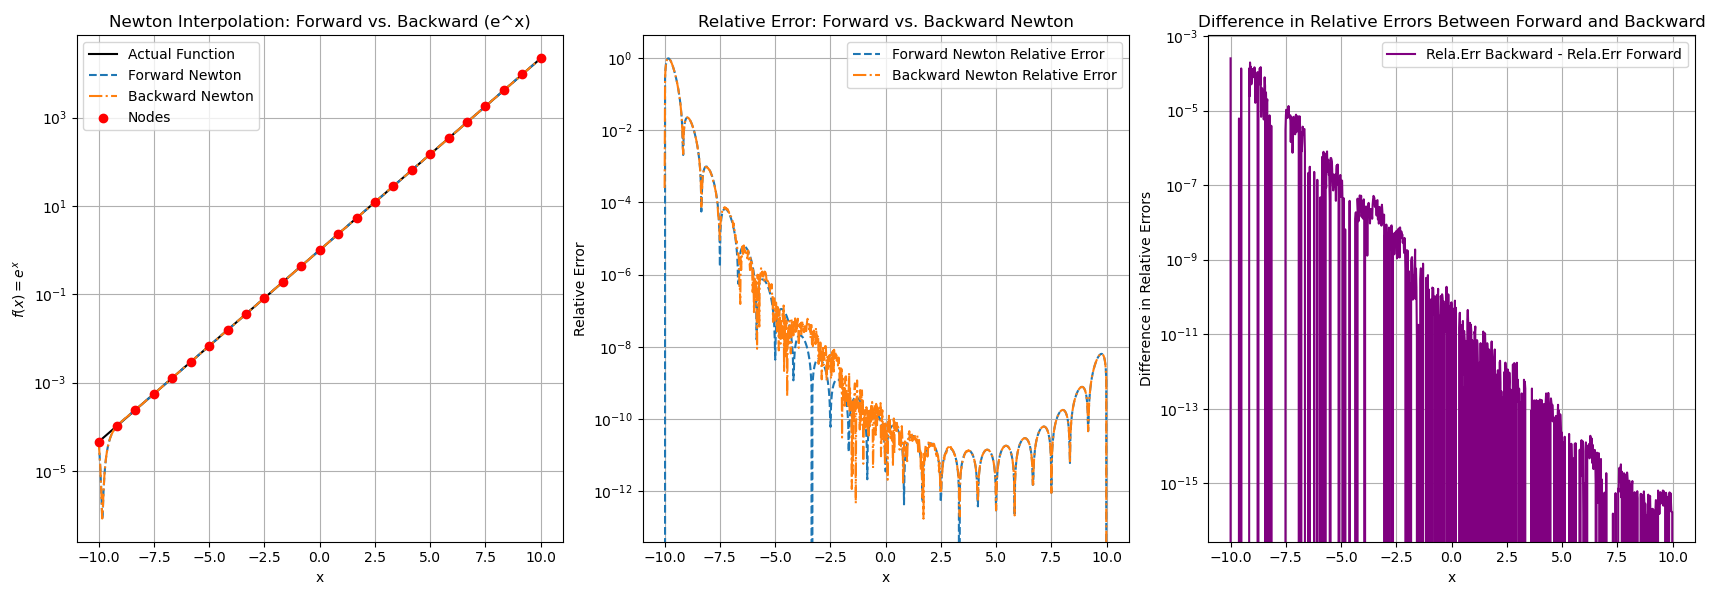
\includegraphics[width=1.0\textwidth]{Problem_3/figs/exp.png}
    \caption{\(\mathrm{e}^x\)实验结果}
\end{figure}
令人惊奇的是,对于病态函数\(\mathrm{e}^x\),顺序插值的效果始终优于逆序插值(表现为子图2中蓝色虚线始终位于橙色虚线下方,子图3中紫色曲线值始终非负)猜测可能是由于逆序差值的系数在计算初期便受到了较大的舍入误差的影响,而这种影响在Horner's Rule中被逐级放大,最终在传播后半段(子图左侧)逐渐显现。

\begin{figure}[H]
    \centering
    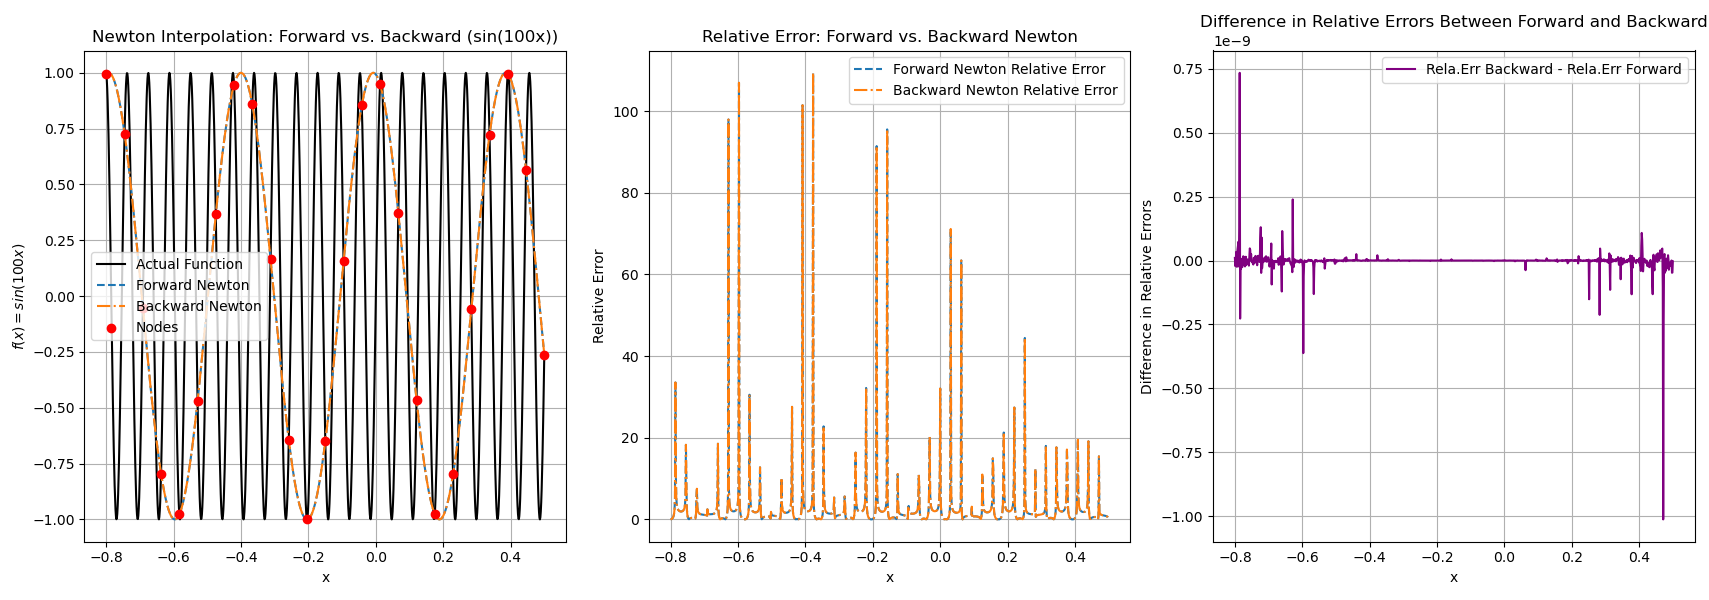
\includegraphics[width=1.0\textwidth]{Problem_3/figs/sin.png}
    \caption{\(\sin(100x)\)实验结果}
\end{figure}

对于高频震荡的病态函数\(\sin(100x)\),逆序差值与顺序差值这对卧龙凤雏,均展现了高达一倍以上的相对误差,相较于\(\mathrm{e}^x\)的结果,更为病态,也符合预期。令人惊喜的是,由于\(\sin(100x)\)本身的对称性与导数有界性,两种差值顺序的优劣对比在区间两端出现了符合预期的差别:在正向传播的末端(子图3右侧),顺序插值的相对误差超过了逆序差值,反之在另一侧,顺序差值结果更优,这符合我们最开始的朴素想法:随着节点的进行,舍入误差的影响逐渐增大,致使区间两侧效果不一,这也提示我们在边界附近应当采集更密的节点,如\ref{sec:problem_1}节中的Chebyshev与Leja节点。

\vspace{5pt}
\end{document}